
\begin{frame}

    \frametitle{Partie III: Les défis liés aux systèmes de recommandations}
    \framesubtitle{Le problème de démarrage à froid (The Cold Start Problem)}

    \begin{figure}
        \centering
        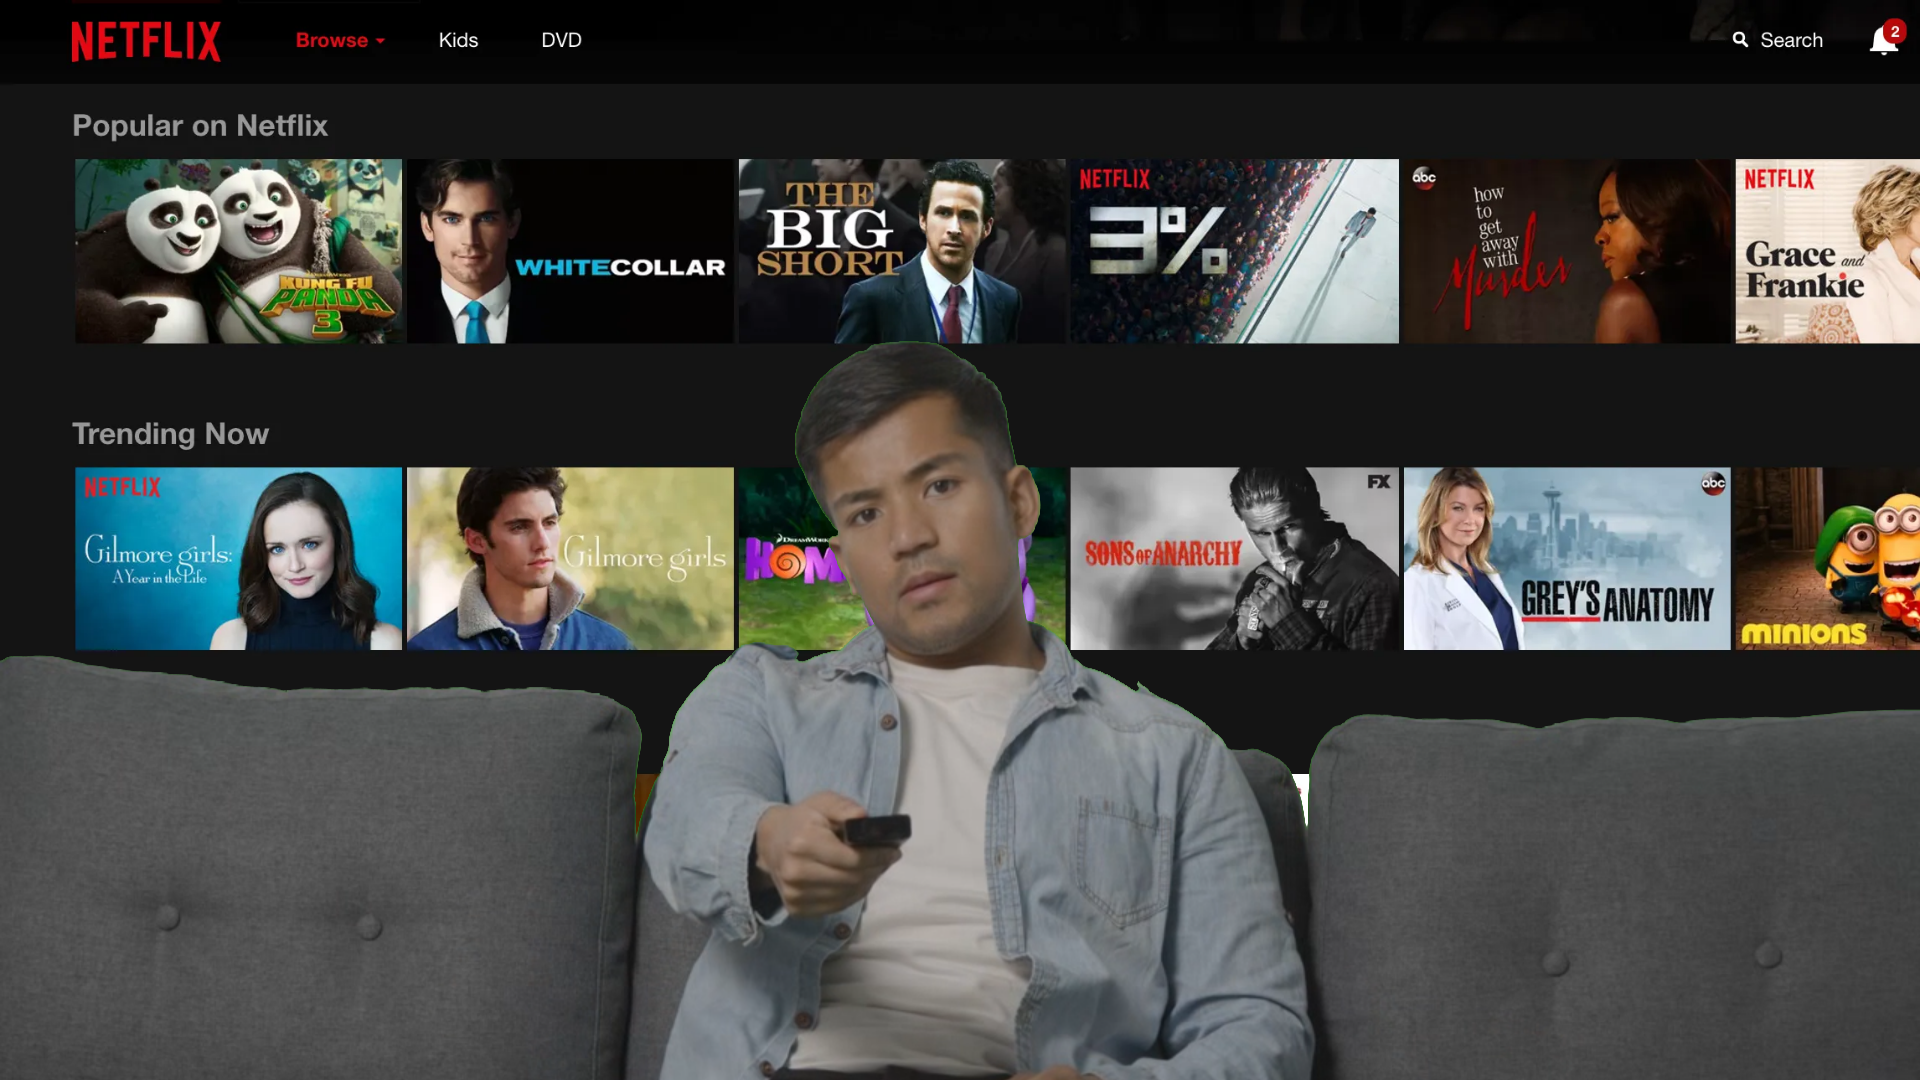
\includegraphics[totalheight=5.5cm]{Images/PartieIII/GuyBrowsingNetflix.png}
        \caption{Chercher un titre à visionner sur Netflix}
    \end{figure}

\end{frame}

\begin{frame}

    \frametitle{Partie III: Les défis liés aux systèmes de recommandations}
    \framesubtitle{Le problème de démarrage à froid (The Cold Start Problem)}

    \begin{figure}
        \[
            \begin{pmatrix}
                5 & 4 & 5 & 1 & 0 \\
                5 & 0 & 3 & 5 & 1 \\
                ? & ? & ? & ? & ? \\
                2 & 1 & 3 & 4 & 4 \\
                1 & 0 & 1 & 2 & 1
            \end{pmatrix}
        \]

    \end{figure}

\end{frame}

\begin{frame}

    \frametitle{Partie III: Les défis liés aux systèmes de recommandations}
    \framesubtitle{Le problème de démarrage à froid (The Cold Start Problem)}

    \begin{figure}
        \centering
        
\includegraphics[totalheight=5.5cm]{Images/PartieIII/NetflixAsking.png}
        \caption{Jump start}
    \end{figure}

\end{frame}

\begin{frame}

    \frametitle{Partie III: Les défis liés aux systèmes de recommandations}

    \begin{figure}
        \centering
        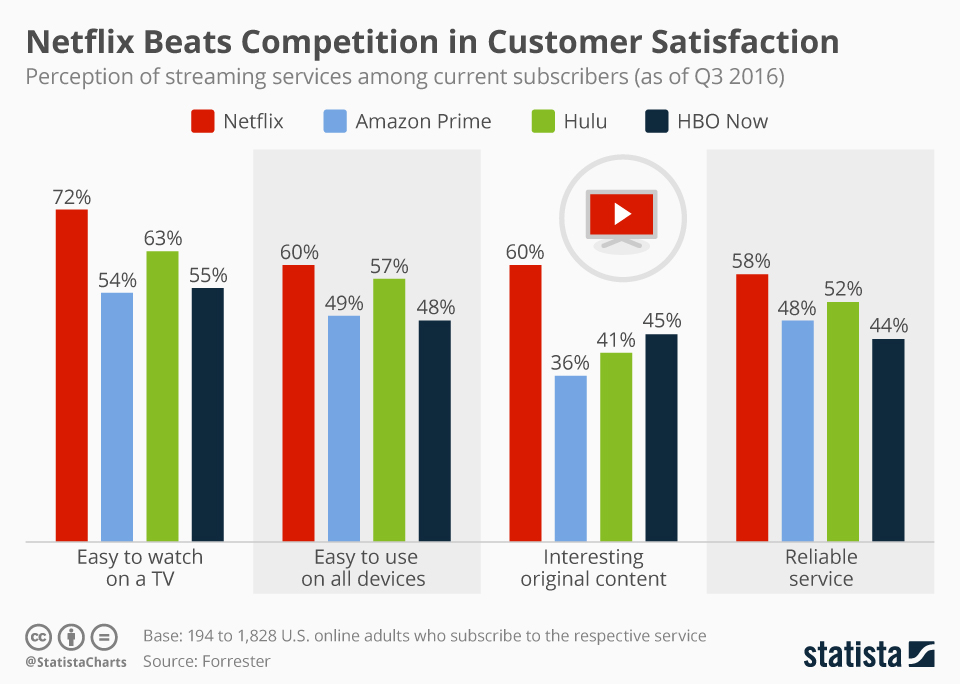
\includegraphics[totalheight=5.5cm]{Images/PartieIII/NetflixCustomerSatisfaction.jpeg}
        \caption{Satisfaction des utilisateurs Netflix}
    \end{figure}

\end{frame}

\begin{frame}

    \frametitle{Partie III: Les défis liés aux systèmes de recommandations}
    \framesubtitle{Les biais liées aux systèmes de recommandation}

    \begin{figure}
        \centering
        \subfigure[Attente]{
\includegraphics[totalheight=5cm]{Images/PartieIII/TargetExpectations.png}}
        \subfigure[Réalité]{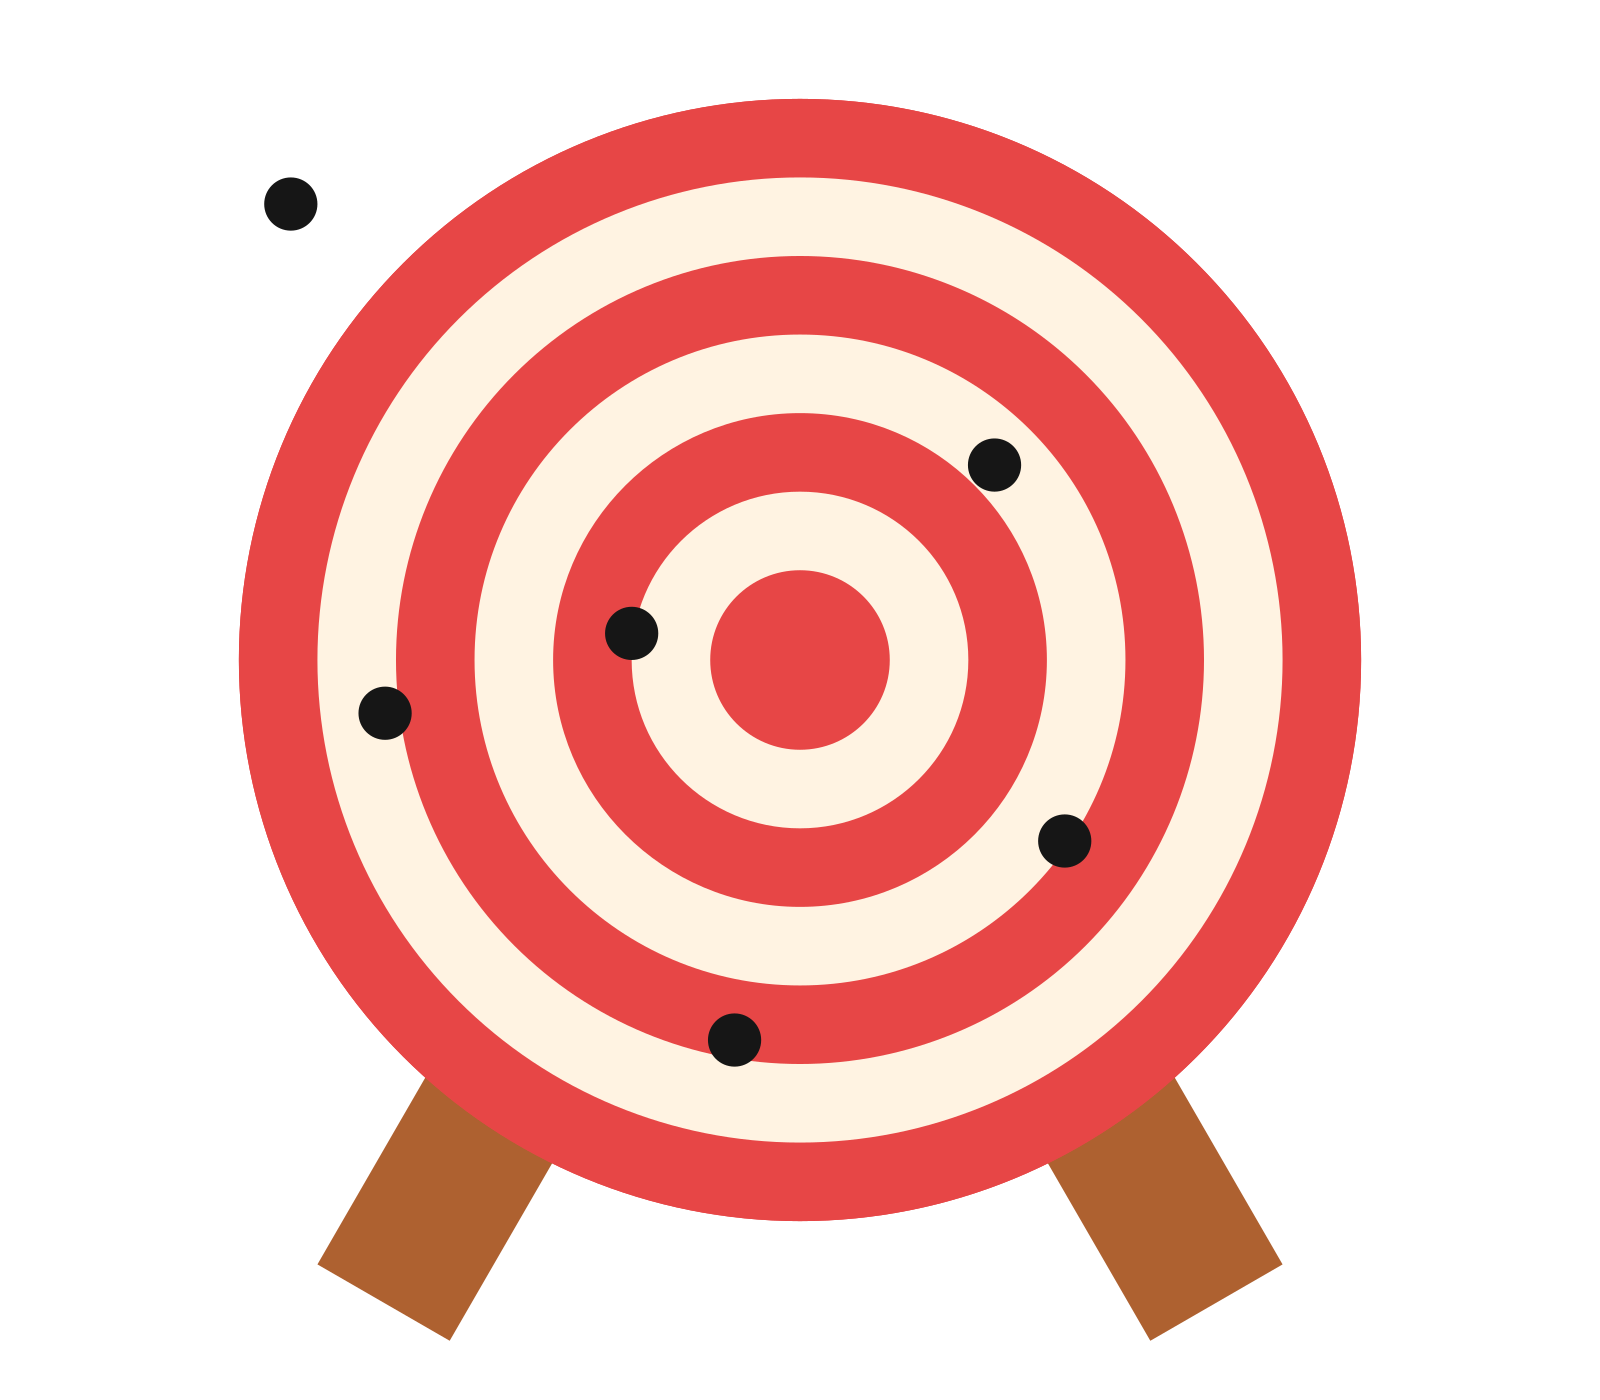
\includegraphics[totalheight=5cm]{Images/PartieIII/TargetReality.png}}
    \end{figure}

\end{frame}

\begin{frame}

    \frametitle{Partie III: Les défis liés aux systèmes de recommandations}
    \framesubtitle{Les biais liées aux systèmes de recommandation}

    \begin{figure}
        \centering
        \subfigure[Différents types de biais]{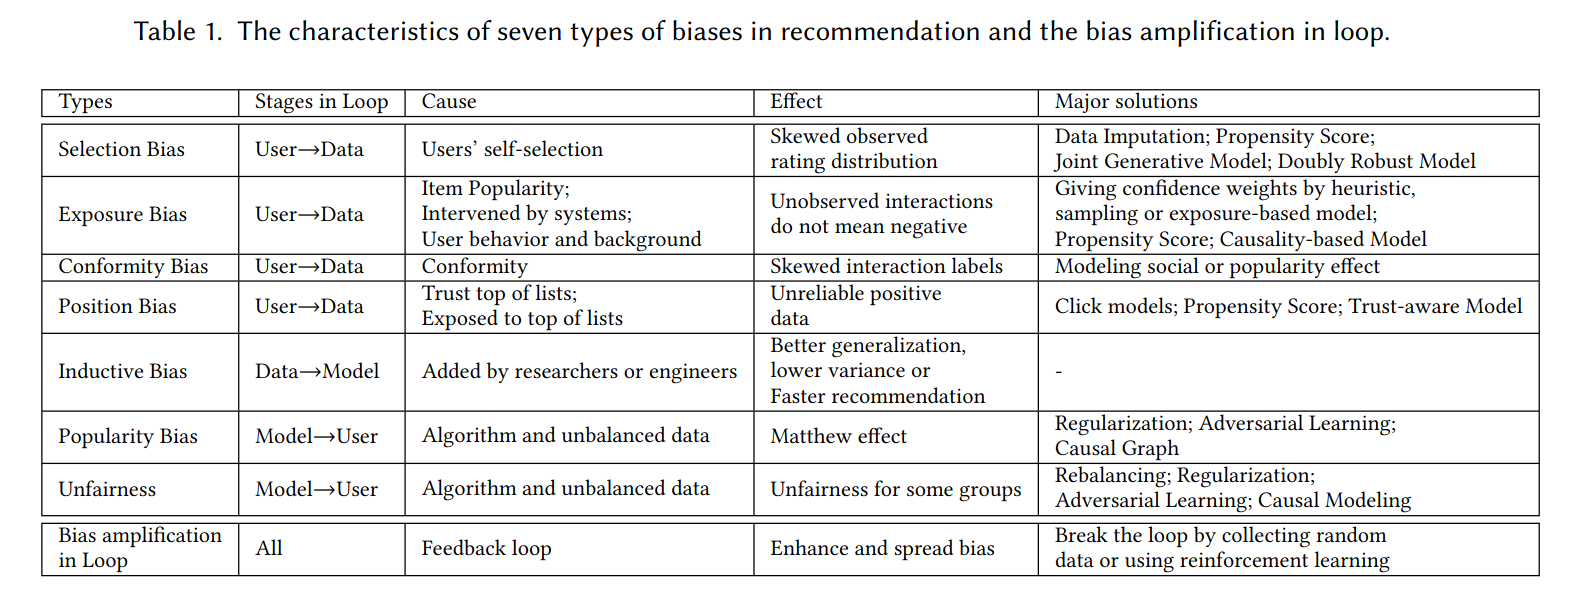
\includegraphics[totalheight=5cm]{Images/PartieIII/BiasTable.png}}
    \end{figure}

\end{frame}

\begin{frame}

    \frametitle{Partie III: Les défis liés aux systèmes de recommandations}
    \framesubtitle{Les biais liées aux systèmes de recommandation}

    \begin{figure}
        \centering
        \subfigure[Différentes méthodes pour débiaiser selon les types de biais]{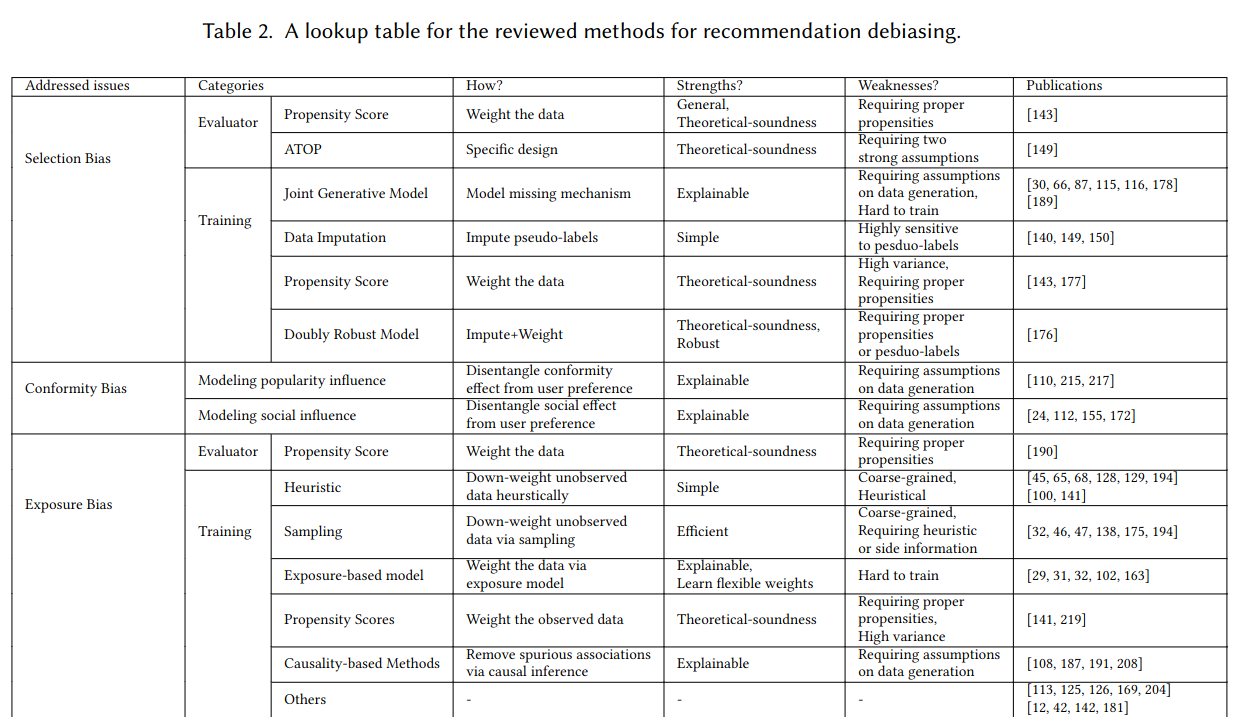
\includegraphics[totalheight=6cm]{Images/PartieIII/DebiasTablePart1.png}}
    \end{figure}

\end{frame}

\begin{frame}

    \frametitle{Partie III: Les défis liés aux systèmes de recommandations}
    \framesubtitle{Les biais liées aux systèmes de recommandation}

    \begin{figure}
        \centering
        \subfigure[Différentes méthodes pour débiaiser selon les types de biais]{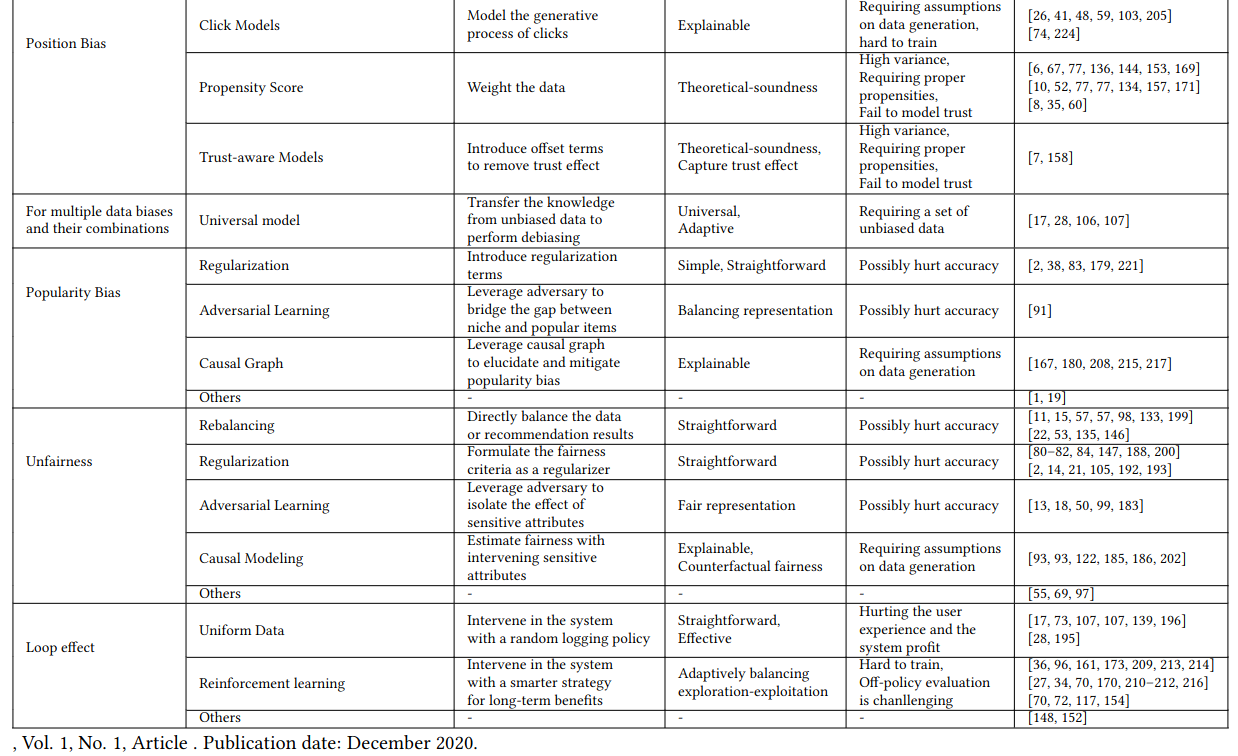
\includegraphics[totalheight=6cm]{Images/PartieIII/DebiasTablePart2.png}}
    \end{figure}

\end{frame}

\begin{frame}

    \frametitle{Partie III: Les défis liés aux systèmes de recommandations}
    \framesubtitle{Les biais liées aux systèmes de recommandation}

    \begin{figure}
        \centering
        \includegraphics[totalheight=5.5cm]{Images/PartieIII/ExposureBias.png}
        \caption{Biais d'exposition}
    \end{figure}

\end{frame}

\begin{frame}

    \frametitle{Partie III: Les défis liés aux systèmes de recommandations}
    \framesubtitle{Les biais liées aux systèmes de recommandation}

    \begin{columns}
        \begin{column}{0.5\textwidth}
            \begin{figure}
                \begin{equation*}
                    R(\hat{Z})=\frac{1}{|\mathcal{U}|} \sum_{u \in \mathcal{U}} \frac{1}{\left|\mathcal{S}_u\right|} \sum_{i \in \mathcal{G}_u} c\left(\hat{Z}_{u i}\right)
                \end{equation*}
                \caption{Correction du biais d'exposition par IPS}
            \end{figure}
        \end{column}

        \begin{column}{0.5\textwidth}
            \begin{figure}
                \begin{equation*}
                    \begin{aligned}
                        \text { AUC }: c\left(\hat{Z}_{u i}\right)      & =1-\frac{\hat{Z}_{u, i}}{|\mathcal{I}|}                                           \\
                        \text { DCG }: c\left(\hat{Z}_{u i}\right)      & =\frac{1}{\log _2\left(\hat{Z}_{u i}+1\right)}                                    \\
                        \text { DCG@k }: c\left(\hat{Z}_{u i}\right)    & =\frac{1\left\{\hat{Z}_{u i} \leq k\right\}}{\log _2\left(\hat{Z}_{u i}+1\right)} \\
                        \text { Recall@k }: c\left(\hat{Z}_{u i}\right) & =1\left\{\hat{Z}_{u i} \leq k\right\}
                    \end{aligned}
                \end{equation*}
                \caption{Différents types de métriques}
            \end{figure}
        \end{column}

    \end{columns}

\end{frame}

\begin{frame}

    \frametitle{Partie III: Les défis liés aux systèmes de recommandations}
    \framesubtitle{Les biais liées aux systèmes de recommandation}

    \begin{figure}
        \centering
        \includegraphics[totalheight=5.5cm]{Images/PartieIII/SelectionBias.png}
        \caption{Biais de sélection}
    \end{figure}

\end{frame}

\begin{frame}

    \frametitle{Partie III: Les défis liés aux systèmes de recommandations}
    \framesubtitle{Les biais liées aux systèmes de recommandation}

    \begin{figure}
        \begin{equation*}
            \hat{H}_{I P S}(\hat{r} \mid \rho)=\frac{1}{|\mathcal{U}||\mathcal{I}|} \sum_{(u, i): s_{u i}=1} \frac{\delta\left(\hat{r}_{u i}, r_{u i}\right)}{\rho_{u i}}
        \end{equation*}
        \caption{Correction du biais de sélection par IPS}
    \end{figure}

\end{frame}

\begin{frame}

    \frametitle{Partie III: Les défis liés aux systèmes de recommandations}
    \framesubtitle{Les biais liées aux systèmes de recommandation}

    \begin{figure}
        \centering
        \includegraphics[totalheight=5.5cm]{Images/PartieIII/PopularityBias.png}
        \caption{Biais de popularité}
    \end{figure}

\end{frame}

\begin{frame}

    \frametitle{Partie III: Les défis liés aux systèmes de recommandations}
    \framesubtitle{Les biais liées aux systèmes de recommandation}

    \begin{figure}
        \begin{equation*}
            \min _{\boldsymbol{\Theta}} \mathcal{L}_{\operatorname{Rec}}+\gamma P C C\left(\widehat{\mathbf{R}}_{+}, p o p(\mathcal{I})\right)^2
        \end{equation*}
        \caption{Correction du biais de popularité par régularisation avec coefficient de corrélation de Pearson}
    \end{figure}

\end{frame}

\begin{frame}

    \frametitle{Partie III: Les défis liés aux systèmes de recommandations}
    \framesubtitle{Les biais liées aux systèmes de recommandation}

    \begin{figure}
        \centering
        \subfigure["Feedback Loop"]{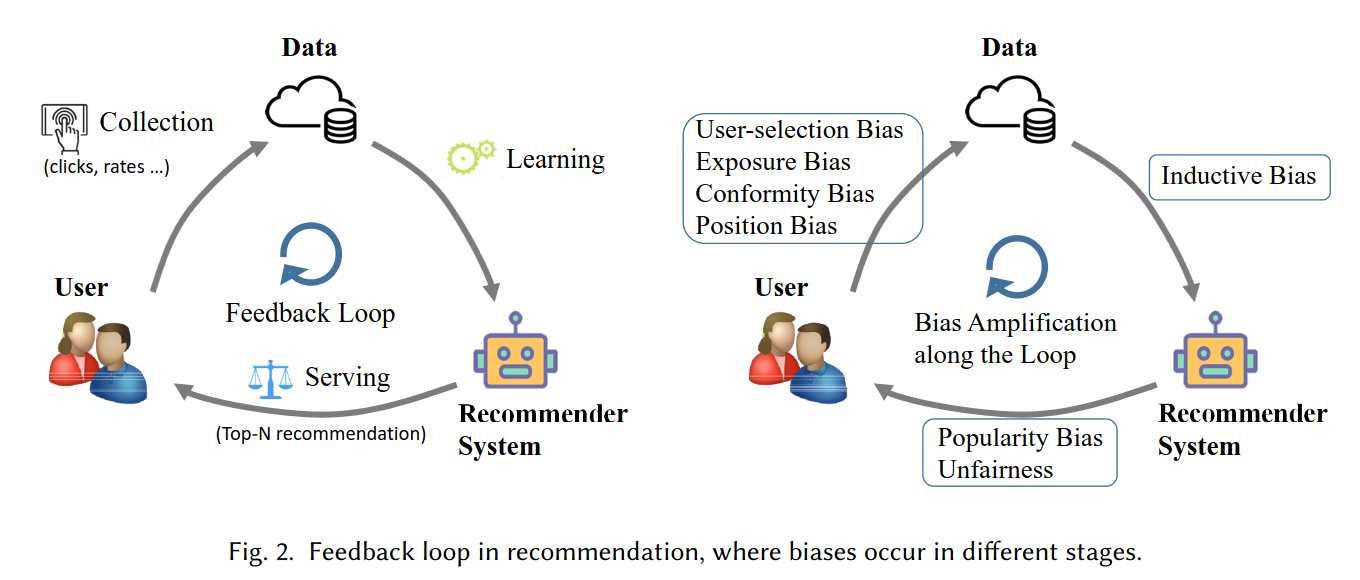
\includegraphics[totalheight=5cm]{Images/PartieIII/FeedbackLoop.png}}
    \end{figure}

\end{frame}

\begin{frame}

    \frametitle{Partie III: Les défis liés aux systèmes de recommandations}
    \framesubtitle{Les biais liées aux systèmes de recommandation}

    \begin{figure}
        \centering
        \subfigure{\includegraphics[width=15cm]{Images/PartieIII/ActionSF.png}}
    \end{figure}

\end{frame}

\begin{frame}

    \frametitle{Partie III: Les défis liés aux systèmes de recommandations}
    \framesubtitle{Les biais liées aux systèmes de recommandation}

    \begin{figure}
        \centering
        \subfigure{\includegraphics[width=15cm]{Images/PartieIII/ActionAction.png}}
    \end{figure}

\end{frame}

\begin{frame}

    \frametitle{Partie III: Les défis liés aux systèmes de recommandations}
    \framesubtitle{Les biais liées aux systèmes de recommandation}

    \begin{figure}
        \centering
        \subfigure{
\includegraphics[width=5cm]{Images/PartieIII/RandomLoggingPolicy.png}}
    \end{figure}

\end{frame}